\documentclass{article}
\usepackage{graphicx} % Required for inserting images
\usepackage[letterpaper,top=2cm,bottom=2cm,left=3cm,right=3cm,marginparwidth=1.75cm]{geometry} % Americanize the paper
\usepackage{float} % To correct image positions
\usepackage{multicol}
\usepackage[colorlinks=true, allcolors=blue]{hyperref} % I want cross referrences

\title{Final Report}
\author{Mark Smith}
\date{\today}

\begin{document}

\maketitle

% \newpage

% \section*{\centering{Abstract}}

% \newpage

% \tableofcontents

% \newpage

\section{Background}

    Solids can be divided into two broad types: crystalline, and amorphous. Crystalline solids have repeating structure that is predictable, and is consistent throughout the entire solid. Amorphous solids have no repeating structures, and have no preferred orientation.
    % For the samples used in this report they are phosphorus diffused into silicon, phosphorus is an amorphous solid, while silicon is a crystalline solid.
    
    X-Ray diffraction (XRD) utilizes x-rays to non-destructively probe the inner atomic layers of materials. In this work it is used to probe different depths of doped silicon to see dopant levels as a function of depth. As the x-ray interacts with the sample it will reflect, refract, and diffract. Diffraction is the process of note, and the only one that will be investigated for this work. 

    When XRD is used on crystalline solids a diffraction pattern will emerge. The spacing between the atoms acts as the slit size that allows for the diffraction interference pattern, in accordance with Bragg's Law ($2d\sin\theta=n\lambda$). There also exist different spacings between atoms that are not nearest neighbors. Each of these different spacings are relegated into planes that act like a diffraction grating, existing for every possible repeating spacing within the atom. All of these in superposition produce a graph that shows sharp peaks correlating directly to the atomic plane's spacing (show in figure \ref{fig:pure crystalline XRD scan}).
    
% Show picture of crystalline XRD pattern
\begin{figure}[H]
    \centering
    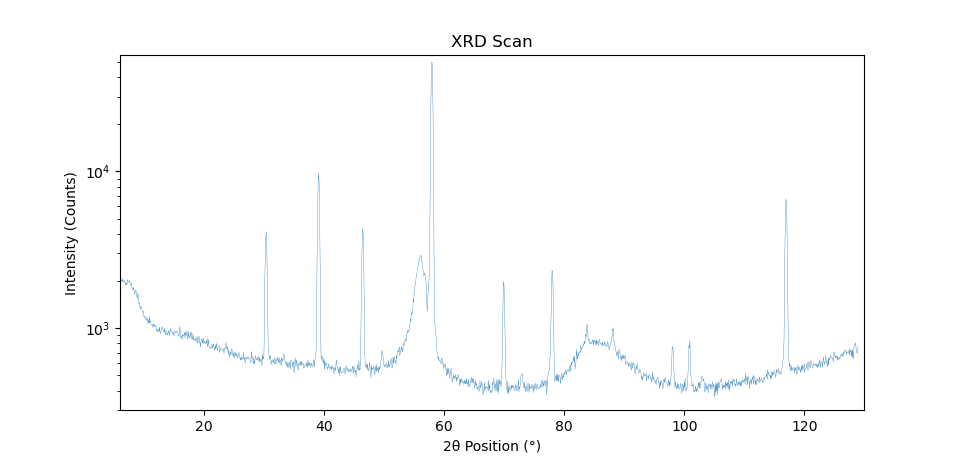
\includegraphics[width=1\linewidth]{crystalline XRD scan.png}
    \caption{Diffractogram of pure crystalline solid}
    \label{fig:pure crystalline XRD scan}
\end{figure}

    Amorphous solids under the x-ray beam behave in a similar manner. The difference being in that because every atom is arranged randomly, there are an infinite number of planes with their own spacing. As shown in figure \ref{fig:pure amorphous XRD scan}, this correlates to a moderately low angle hump (called an amorphous hump) with all spacings that would correlate to higher angled peaks being nonexistent because of deconstructive interference.

% Show picture of amorphous XRD pattern
\begin{figure}[H]
    \centering
    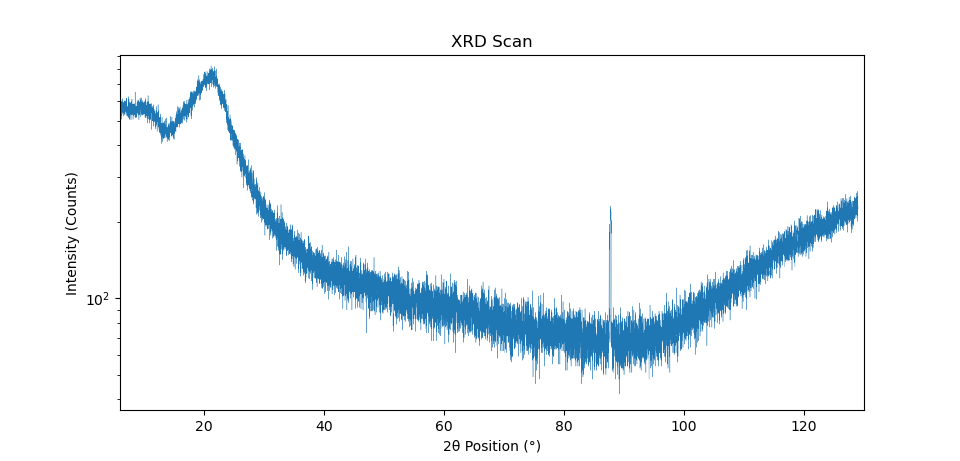
\includegraphics[width=1\linewidth]{amorphous XRD scan.png}
    \caption{Diffractogram of pure amorphous solid}
    \label{fig:pure amorphous XRD scan}
\end{figure}

    The materials analyzed in this work are silicon doped with phosphorous, silicon doped with boron, and pure silicon. The first two materials will be best thought of as a gradient from pure phosphorous or boron to pure silicon from top to bottom. Silicon is a crystalline material, while phosphorous and boron are amorphous. This means that the diffractogram will be a superposition of an amorphous diffractogram on a crystalline diffractogram. The silicon sample was only used to verify the amorphous hump was present on the diffractograms.

    The XRD process used to incrementally probe deeper depths is called grazing incidence x-ray diffraction (GIXRD, also called glancing incidence x-ray diffraction). Using this method the XRD will hold the incident beam at a fixed angle (called omega ($\omega$)), while the diffracted beam side moves from a starting angle to an end angle. The detector is used in a 0D mode that simply counts all the x-rays that interact with it. The angle the counts correspond to is the angle the incident beam is added to the current diffracted beam angle all multiplied by 2: ($2(\omega+\theta)$). After the scan finishes a new scan is started with a different incident angle to probe a different depth.

% Picture of GIXRD schematic
\begin{figure}[H]
    \centering
    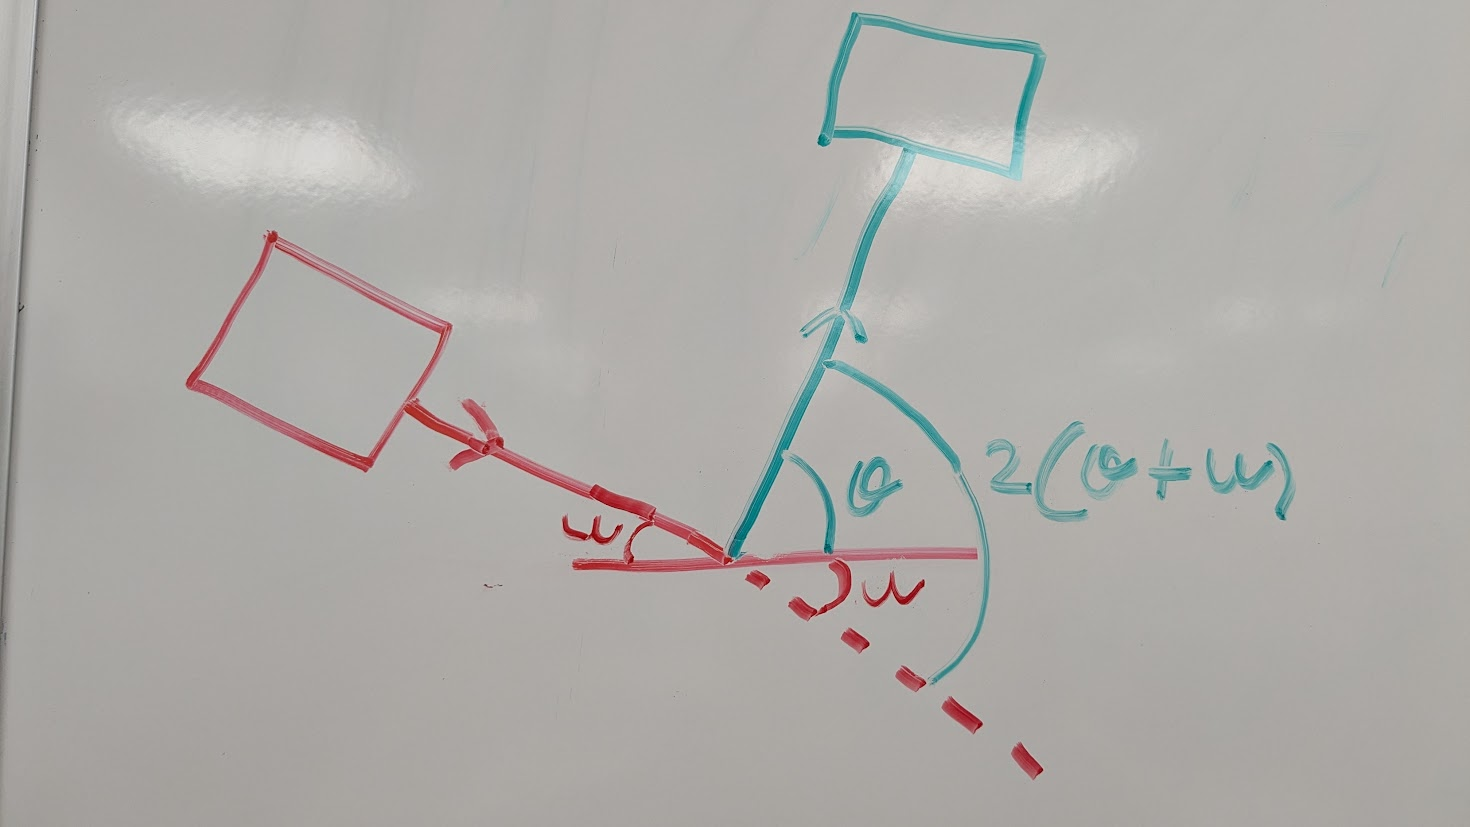
\includegraphics[width=.75\linewidth]{2theta scan diagram.jpg}
    \caption{Diagram of XRD using GIXRD}
    \label{fig:GIXRD diagram}
\end{figure}

    The different incident angles probe different depths due to the different path lengths they provide the x-rays as they interact with the samples. This is due to the exponential attenuation of intensity as the beam travels given by this equation: $I(y)=I_0e^{-\alpha y}$ with $\alpha=2\omega n_I/c$. With the complex index of refraction ($n_I$) strongly dependent on wavelength. The x-ray source is copper, producing $K_\alpha$, and $K_\beta$ in most abundance. Since one wavelength provides the most uniformity on the diffractogram, the incident beam optics include a filter to limit the unnecessary wavelength. $K_\alpha$ is what is most common, so the $K_\beta$ gets mostly filtered out by a nickel filter. This results in a x-ray beam that has a wavelength of 1.54\AA \space (uniformity in the wavelength is also necessary for Bragg's law).
    
\section{Methods}

    Three different methods for determining relative percentages of the dopant in the substrate are used. The methods are: 1. Take the ratio of the max peak intensity, 2. Fit the peaks to a Gaussian curve, and find the integrated area, 3. Perform a summation to find the numerical integral. These methods are predicated on certain assumption. The mixture of the probed depth is uniform, which is a known simplification of how the diffused dopants actually spread. An analysis to correct this has been tried, but better data is needed for it to be effective. The intensity of the x-ray is also assumed to have attenuated by 90\%, and all relevant data comes from that.

    \subsection*{Method 1: Ratio}

        With this method the program takes the max intensity of the amorphous hump, and the max intensity of the most intense crystalline peak, and takes the ratio of them. This ratio is then the relative percentages of the dopant and substrate.

    \subsection*{Method 2: Curve Fitting}

        This method takes the position and intensity values as the x and y inputs of scipy's curve\_fit function. It then outputs the best fit for amplitude, mean, standard deviation, and a background value. The function then gets integrated, and the ratio of the areas are taken.

    \subsection*{Method 3: Summation}

        This is an integral method as in method 2, but instead of fitting the data to a curve the data is integrated using discrete methods. The dx is the same for all points, so it is ignored with the foresight that it will be divided out. The sum is of all the intensity values for the peak or hump. A ratio is then taken from these sums.

\section{Results}
    
    \begin{figure}[H]
        \centering
        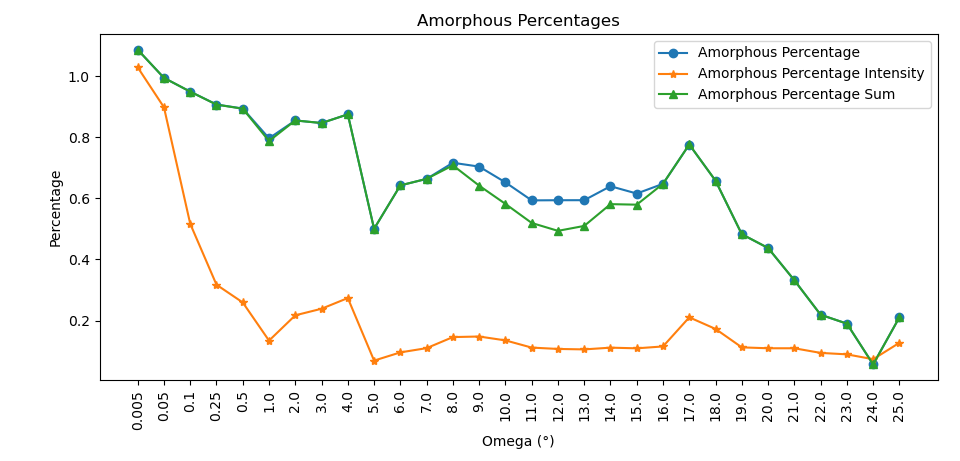
\includegraphics[width=.9\linewidth]{Mixture Line Graph (amorphous)_final.png}
        \caption{Percent amorphous at selected omegas}
        \label{fig:line graph amorphous}
    \end{figure}

    Figure \ref{fig:line graph amorphous} provides a concise overview of how the dopant and substrate mixture change with omega. All three methods show the amorphous percent decreases with depth, which is to be expected. The curve fitting and summation method provide excellent agreement with each other.
        
    \begin{figure}[H]
        \centering
        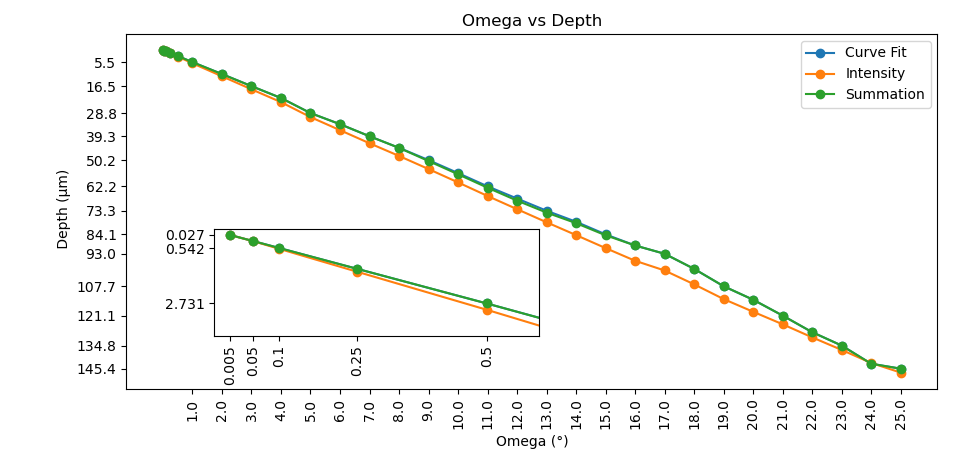
\includegraphics[width=1\linewidth]{Depth vs Omega.png}
        \caption{Depth vs omega for the three methods}
        \label{fig:depth vs omega}
    \end{figure}
    
    Figure \ref{fig:depth vs omega} shows the depth that correlates with the three methods. The methods have a close agreement, with the curve fit and summation method being right on top of each other.

\section{Conclusion}

    Using GIXRD to determine relative composition of samples led to three analysis methods. Two of the methods utilized integration, and their results are closer together. One method used peak intensity ratios, and provides results that differ noticeably more. All three methods provide reasonable agreement as to the depth that each omega probed. Using GIXRD to see relative mixture amount dependent on depth has been shown to be useful, keeping in mind the limitations given by the assumptions.
    
\section{References}

% \begin{small}
    \begingroup
    \makeatletter
    \@totalleftmargin=-1cm
	\begin{verbatim}
import matplotlib.pyplot as plt # Used for plotting
import numpy as np # Used for arrays, and some math functions
import pandas as pd # Used for reading and writing files
import os # Used for file handling
from scipy.optimize import curve_fit # Used for fitting functions to data
from scipy.stats import chi2 # Used for chi squared probability calculations
import traceback # Used for error handling
import sys # Used for error handling
import re # Used to extract omega from file names
import sympy as sp # Used for uncertainty calculations
np.set_printoptions(threshold=np.inf) # Forces numpy to print everything in an array. This is useful for exporting everything to a file
"""
This script processes X-ray diffraction (XRD) data to fit peaks, calculate areas, and analyze sample depth.
It reads scan data from CSV files, fits Gaussian functions to the peaks, calculates the area under the peaks,
and determines the mixture of amorphous and crystalline phases. It also calculates the sample depth based on the peak areas.
It includes functions to read data, fit peaks, calculate areas, and analyze sample depth. It then exports the data to excel.

Mark Smith
"""

def XRD_Data_Dictionary(path_name: str): # Gets position and intensity from file to a dictionary
    """
    Reads XRD data from a specified path and returns a dictionary with the data.

    Parameters:
        path_name (str): The path to the directory containing the XRD data files.

    Returns:
        dict: A dictionary where keys are file names, and values are position and intensity.
    """
    xrd_data = {} # Initialize an empty dictionary to store the data

    os.chdir(path_name) # Change the current working directory to the specified path
    
    # Inputs to get from the user (or to hardcode in options)
    omega_in_file_name = 'y' # input('Are the omega values in the file names followed by a w? (y/n): ').strip().lower() # This allows for automatic omega extraction (highly reccommended)
    normalize_choice = 'n' # input("Do you want to normalize the intensity data? (y/n): ").strip().lower()  # Ask the user if they want to normalize the intensity data
    smooth = 'n' # input("Do you want to smooth the data? (y/n): ").strip().lower()  # Ask the user if they want to smooth the data
    if smooth == 'y':
        how_smooth = 25 # int(input("How many points do you want to smooth over? (e.g., 25): "))  # Ask the user how many points to smooth over
    
    for file in os.listdir(path_name): # Iterate through each file in the directory
        if file.endswith('.csv'): # Process only CSV files
            try:
                scan = pd.read_csv(file, index_col=0) # Read the CSV file into a DataFrame

                intensity = scan['Intensity [Counts]'].to_numpy()  # Get the intensity data from the CSV file
                position = scan['Pos. [°2θ]'].to_numpy()  # Get the position data from the CSV file

                # Smooth data                
                if smooth == 'y':
                    i = 0
                    intensity_smooth = []
                    position_smooth = []
                    while i < len(intensity)-how_smooth:
                        intensity_sum = 0
                        position_sum = 0
                        for j in range(how_smooth):
                            intensity_sum += intensity[i+j]
                            position_sum += position[i+j]
                        intensity_smooth.append(intensity_sum/how_smooth)
                        position_smooth.append(position_sum/how_smooth)
                        i += how_smooth
                else:
                    intensity_smooth = intensity
                    position_smooth = position
                
                if omega_in_file_name == 'y':
                    # Extract omega using regex (matches numbers with optional decimal before 'w')
                    match = re.search(r'([0-9.]+)w', file)
                    if match:
                        omega = float(match.group(1))
                    else:
                        print(f"Could not extract omega from filename: {file}")
                        continue  # Skip this file if omega can't be extracted
                else:
                    omega = float(input(f'Input the omega for this file {file}: '))
                
                if normalize_choice == 'y':
                    intensity = intensity/max(intensity)  # Normalize the intensity data to the maximum value

                xrd_data[file] = {'omega': omega, 'Position': np.array(position_smooth), 'Intensity': np.array(intensity_smooth)} #, 'Time Step': position_smooth[1]-position_smooth[0]}  # Store the data in the dictionary

            except Exception as e: # Skips non scan files
                print(f"Error processing file {file}: {e}")
                pass

    # Sort the dictionary by omega in descending order
    sorted_data = dict(sorted(xrd_data.items(), key=lambda item: item[1]['omega'], reverse=True))
    print('\n')
    return sorted_data

def Length_Peak(data: dict): # Just gets the peak ranges
    """
    Prompts the user to input the amorphous and crystalline ranges for each file in 
    the data dictionary.

    Parameters:
        data (dict): A dictionary containing XRD data with file names as keys and 
            position/intensity as values.

    Returns:
        dict: The updated dictionary with amorphous and crystalline ranges added for each file.
    """
    manual_input = 'no' # input("Do you want to manually input the ranges? (yes/no): ").strip().lower()  # Ask the user if they want to manually input the ranges

    if manual_input == 'no':
        peak_range_file = 'Peak_Ranges.txt' # input("Enter the file name containing the peak ranges (e.g., 'peak_ranges.txt'): ")
        peak_ranges = pd.read_csv(peak_range_file)  # Read the peak ranges from the specified file

    for file_name in data.keys():

        if manual_input == 'yes':
            print(f"Processing file: {file_name}")
            amorphous_range = input("Enter the amorphous range (e.g., 20-30): ")
            amorphous_range = [float(x) for x in amorphous_range.split('-')]  # Convert the input range to a list of floats

            crystalline_range = input("Enter the crystalline range (e.g., 30-40): ")
            crystalline_range = [float(x) for x in crystalline_range.split('-')]  # Convert the input range to a list of floats

            print('\n')

        else:
            omega = data[file_name]['omega']  # Get the omega value from the data dictionary
            file_index = peak_ranges.index[peak_ranges['Omega'] == omega]  # Find the index of the file in the peak ranges DataFrame

            amorphous_range = [float(x) for x in peak_ranges.loc[file_index, ' Amorphous Range'].values[0].split('-')]  # Get the amorphous range from the DataFrame
            crystalline_range = [float(x) for x in peak_ranges.loc[file_index, ' Crystalline Range'].values[0].split('-')]  # Get the crystalline range from the DataFrame

        data[file_name]['amorphous_range'] = amorphous_range
        data[file_name]['crystalline_range'] = crystalline_range

    return data

def Gaussian_function(current_x_value: float, amplitude: float, mean: float, standard_deviation: float, background: float = 0): # Function to fit to
    """
    Calculates the Gaussian function value for a given x value.

    Parameters:
        current_x_value (float): The x value at which to evaluate the Gaussian function.

        amplitude (float): The amplitude of the Gaussian peak.

        mean (float): The mean (center) of the Gaussian peak.

        standard_deviation (float): The standard deviation of the Gaussian peak.

        background (float): The background value to be added to the Gaussian function.

    Returns:
        float: The value of the Gaussian function at the given x value.
    """

    func = amplitude*np.exp(-.5*((current_x_value-mean)/standard_deviation)**2)/(standard_deviation*np.sqrt(2*np.pi))+ background  # Calculate the Gaussian function value

    return func

def Peak_fit(data: dict, background: bool = True): # Fit the peaks to a Gaussian function
    """
    Fits the peaks in the XRD data based on the provided ranges.

    Parameters:
        data (dict): A dictionary containing XRD data with file names as keys and 
            position/intensity as values, including amorphous and crystalline ranges.

    Returns:
        dict: An updated dictionary with fitted peak areas for each file.
    """

    for file_name, file_data in list(data.items()): # Iterate through each file in the data dictionary using key and value
        try:
            # Unpack the values from the file data
            position = file_data['Position']
            intensity = file_data['Intensity']
            amorphous_range_start_user, amorphous_range_end_user = file_data['amorphous_range']
            crystalline_range_start_user, crystalline_range_end_user = file_data['crystalline_range']

            # Pull out the actual data for the amorphous and crystalline peaks
            amorphous_mask = ((position >= amorphous_range_start_user) & (position <= amorphous_range_end_user) & ~((position > crystalline_range_start_user) & (position < crystalline_range_end_user)))
            crystalline_mask = ((position >= crystalline_range_start_user) & (position <= crystalline_range_end_user))

            x_values_amorphous = position[amorphous_mask]
            y_values_amorphous = intensity[amorphous_mask]

            x_values_crystalline = position[crystalline_mask]
            y_values_crystalline = intensity[crystalline_mask]

            # Subtract background when needed
            if background == False:
                y_values_amorphous = y_values_amorphous - data[file_name]['amorphous_fit_background'] # Get the intensity values for the amorphous range
                y_values_crystalline = y_values_crystalline - data[file_name]['crystalline_fit_background'] # Get the intensity values for the crystalline range
            
            # Get guesses for the Gaussian parameters
            guess_background = min(intensity)  # Guess the background for the peaks
            
            guess_amplitude_amorphous = y_values_amorphous.max() # Guess the amplitude for the amorphous peak
            guess_mean_amorphous = x_values_amorphous.mean() # Guess the mean for the amorphous peak
            guess_std_amorphous = x_values_amorphous.std()/2  # Guess the standard deviation for the amorphous peak
            guess_amorphous = [guess_amplitude_amorphous, guess_mean_amorphous, guess_std_amorphous, guess_background]  # Create a list of guesses for the amorphous peak

            guess_amplitude_crystalline = y_values_crystalline.max() # Guess the amplitude for the crystalline peak
            guess_mean_crystalline = x_values_crystalline.mean() # Guess the mean for the crystalline peak
            guess_std_crystalline = x_values_crystalline.std()/2
            guess_crystalline = [guess_amplitude_crystalline, guess_mean_crystalline, guess_std_crystalline, guess_background]

            if background == False:
                guess_amorphous = guess_amorphous[:-1]  # Remove the background guess for the amorphous peak
                guess_crystalline = guess_crystalline[:-1]  # Remove the background guess for the crystalline peak

            # Fit the Gaussian function to the data
            fit_amorphous, error_amorphous = curve_fit(Gaussian_function,x_values_amorphous,y_values_amorphous,p0=guess_amorphous)
            uncert_amorphous = np.sqrt(np.diag(error_amorphous))

            fit_crystalline, error_crystalline = curve_fit(Gaussian_function,x_values_crystalline,y_values_crystalline,p0=guess_crystalline)
            uncert_crystalline = np.sqrt(np.diag(error_crystalline))

            # Check the fit of the fit (chi-squared test)
            nu_amorphous = len(x_values_amorphous)-3
            chi_squared_amorphous = np.sum(((y_values_amorphous - Gaussian_function(x_values_amorphous, *fit_amorphous))**2 / y_values_amorphous))
            p_value_amorphous = chi2.sf(chi_squared_amorphous, nu_amorphous)

            nu_crystalline = len(x_values_crystalline)-3
            chi_squared_crystalline = np.sum(((y_values_crystalline - Gaussian_function(x_values_crystalline, *fit_crystalline))**2 / y_values_crystalline))
            p_value_crystalline = chi2.sf(chi_squared_crystalline, nu_crystalline)

            # Store the fitted parameters and uncertainties in the data dictionary
            data[file_name]['amorphous_fit_amplitude'] = fit_amorphous[0]
            data[file_name]['amorphous_fit_amplitude_uncertainty'] = uncert_amorphous[0]
            data[file_name]['amorphous_fit_mean'] = fit_amorphous[1]
            data[file_name]['amorphous_fit_mean_uncertainty'] = uncert_amorphous[1]
            data[file_name]['amorphous_fit_std_dev'] = fit_amorphous[2]
            data[file_name]['amorphous_fit_std_dev_uncertainty'] = uncert_amorphous[2]
            if background == True:
                data[file_name]['amorphous_fit_background'] = fit_amorphous[3]
                data[file_name]['amorphous_fit_background_uncertainty'] = uncert_amorphous[3]
                data[file_name]['chi_squared_amorphous'] = chi_squared_amorphous
                data[file_name]['amorphous_nu'] = nu_amorphous
                data[file_name]['chi_squared_amorphous_p'] = p_value_amorphous
            data[file_name]['amorphous_fit_amorphous_x_range_used'] = x_values_amorphous
            data[file_name]['amorphous_fit_amorphous_y_range_used'] = y_values_amorphous

            data[file_name]['crystalline_fit_amplitude'] = fit_crystalline[0]
            data[file_name]['crystalline_fit_amplitude_uncertainty'] = uncert_crystalline[0]
            data[file_name]['crystalline_fit_mean'] = fit_crystalline[1]
            data[file_name]['crystalline_fit_mean_uncertainty'] = uncert_crystalline[1]
            data[file_name]['crystalline_fit_std_dev'] = fit_crystalline[2]
            data[file_name]['crystalline_fit_std_dev_uncertainty'] = uncert_crystalline[2]
            if background == True:
                data[file_name]['crystalline_fit_background'] = fit_crystalline[3]
                data[file_name]['crystalline_fit_background_uncertainty'] = uncert_crystalline[3]
                data[file_name]['chi_squared_crystalline'] = chi_squared_crystalline
                data[file_name]['crystalline_nu'] = nu_crystalline
                data[file_name]['chi_squared_crystalline_p'] = p_value_crystalline
            data[file_name]['crystalline_fit_crystalline_x_range_used'] = x_values_crystalline
            data[file_name]['crystalline_fit_crystalline_y_range_used'] = y_values_crystalline

            # Store max values for the peaks
            data[file_name]['max_amorphous'] = max(y_values_amorphous)  # Store the maximum value of the amorphous peak
            data[file_name]['max_crystalline'] = max(y_values_crystalline) # Store the maximum value of the crystalline peak

        except RuntimeError as e: # This error will happen when a fit cannot be calculated
            print(f"{file_name} was not able to be fitted")
            print(e)

            # Determine what caused the error
            my_script = os.path.basename(__file__)
            exc_type, exc_value, exc_tb = sys.exc_info()
            tb = traceback.extract_tb(exc_tb)
            for frame in reversed(tb):
                if os.path.basename(frame.filename) == my_script:

                    if 'amorphous' in frame.line: 
                        print("The amorphous range caused the error")
                    elif 'crystalline' in frame.line:
                        print("The crystalline range caused the error")
                    else:
                        print("Unforseen error occured on line ", frame.lineno)
                        # print(f"Error occurred on line {frame.lineno}: {frame.line}") # This will show the line where the error happened

                    break

            data.pop(file_name, None) # Get rid of the file for analysis

            show_plot = input("Would you like to see the plot to see potential issues? (y/n): ").strip().lower()
            if show_plot == 'y':
                plt.title(file_name)
                plt.plot(position, intensity)
                plt.plot(x_values_amorphous, y_values_amorphous, 'ko')
                plt.plot(x_values_crystalline, y_values_crystalline, 'bo')
                plt.yscale('log')
                plt.show()

            print('\n') # Helps distinguish the next print group

    return data

def Peak_Area_Calculation(data: dict):
    """
    Calculates the area under the fitted peaks for each file in the data dictionary.

    Parameters:
        data (dict): A dictionary containing XRD data with fitted peak parameters.

    Returns:
        dict: An updated dictionary with calculated peak areas for each file.
    """

    for file_name, file_data in data.items():
        # Calculate the area under the amorphous peak
        amplitude_amorphous = file_data['amorphous_fit_amplitude']
        mean_amorphous = file_data['amorphous_fit_mean']
        std_dev_amorphous = file_data['amorphous_fit_std_dev']
        background_amorphous = file_data['amorphous_fit_background']
        x_values_amorphous = file_data['amorphous_fit_amorphous_x_range_used']
        # area_amorphous = np.trapz(Gaussian_function(x_values_amorphous, amplitude_amorphous, mean_amorphous, std_dev_amorphous, background_amorphous), x=x_values_amorphous)  # Calculate the area under the amorphous peak
        area_amorphous = np.trapz(Gaussian_function(x_values_amorphous, amplitude_amorphous, mean_amorphous, std_dev_amorphous), x=x_values_amorphous)  # Calculate the area under the amorphous peak

        # Calculate the area under the crystalline peak
        amplitude_crystalline = file_data['crystalline_fit_amplitude']
        mean_crystalline = file_data['crystalline_fit_mean']
        std_dev_crystalline = file_data['crystalline_fit_std_dev']
        background_crystalline = file_data['crystalline_fit_background']
        x_values_crystalline = file_data['crystalline_fit_crystalline_x_range_used']
        # area_crystalline = np.trapz(Gaussian_function(x_values_crystalline, amplitude_crystalline, mean_crystalline, std_dev_crystalline, background_crystalline), x=x_values_crystalline) # Calculate the area under the crystalline peak
        area_crystalline = np.trapz(Gaussian_function(x_values_crystalline, amplitude_crystalline, mean_crystalline, std_dev_crystalline), x=x_values_crystalline) # Calculate the area under the crystalline peak

        amorphous_intensity_sum = sum(file_data['amorphous_fit_amorphous_y_range_used'])  # Sum the intensity values for the amorphous peak
        crystalline_intensity_sum = sum(file_data['crystalline_fit_crystalline_y_range_used'])  # Sum the intensity values for the crystalline peak
        # area_amorphous = amorphous_intensity_sum/(amorphous_intensity_sum+crystalline_intensity_sum)
        # area_crystalline = crystalline_intensity_sum/(amorphous_intensity_sum+crystalline_intensity_sum)

        # Store the areas in the data dictionary
        data[file_name]['amorphous_area'] = area_amorphous
        # data[file_name]['amorphous_area_rate'] = area_amorphous/data[file_name]['Time Step']
        data[file_name]['crystalline_area'] = area_crystalline
        data[file_name]['amorphous_area_sum'] = amorphous_intensity_sum
        data[file_name]['crystalline_area_sum'] = crystalline_intensity_sum

    return data

def Peak_Mixture_Calculation(data: dict): # Calculates the mixture fraction from amorphous and crystalline areas
    """
    Calculates the mixture of amorphous and crystalline areas for each file in the data dictionary.

    Parameters:
        data (dict): A dictionary containing XRD data with calculated peak areas.

    Returns:
        dict: An updated dictionary with calculated peak mixtures for each file.
    """

    for file_name, file_data in data.items():
        # Unpack needed values from data
        area_amorphous = file_data['amorphous_area']
        area_crystalline = file_data['crystalline_area']
        area_amorphous_sum = file_data['amorphous_area_sum']
        area_crystalline_sum = file_data['crystalline_area_sum']

        amorphous_percentage = area_amorphous / (area_amorphous + area_crystalline)  # Calculate the amorphous percentage
        crystalline_percentage = area_crystalline / (area_amorphous + area_crystalline)  # Calculate the crystalline percentage

        data[file_name]['amorphous_percentage'] = amorphous_percentage
        data[file_name]['crystalline_percentage'] = crystalline_percentage
        data[file_name]['amorphous_percentage_intensity'] = file_data['max_amorphous'] / (file_data['max_amorphous'] + file_data['max_crystalline'])  # Calculate the amorphous percentage based on intensity
        data[file_name]['crystalline_percentage_intensity'] = file_data['max_crystalline'] / (file_data['max_amorphous'] + file_data['max_crystalline'])
        data[file_name]['amorphous_percentage_sum'] = area_amorphous_sum/(area_amorphous_sum+area_crystalline_sum)
        data[file_name]['crystalline_percentage_sum'] = area_crystalline_sum/(area_amorphous_sum+area_crystalline_sum)

    return data

def Sample_Depth_Analysis(data: dict):
    """
    Analyzes the sample depth based on the calculated peak areas.

    Parameters:
        data (dict): A dictionary containing XRD data with calculated peak mixtures.

    Returns:
        dict: An updated dictionary with sample depth analysis results for each file.
    """

    def skin_depth(alpha: float): # Skin depth calculation (only used in this function)
        """
        Calculate the skin depth for a given attenuation coefficient.

        Parameters:
            alpha (float): Attenuation coefficient in m^-1.

        Returns:
            float: Skin depth in meters.
        """
        return 1 / alpha  # Skin depth in meters

    def real_depth(skin_depth: float, ω: float): # Real depth calculation (only used in this function)
        """
        Calculate the real depth for a given attenuation coefficient and angle.
        This calculates the depth at which 90% of the signal is attenuated.

        Parameters:
            skin_depth (float): Skin depth of mixture.
            ω (float): Angle in degrees.

        Returns:
            float: Real depth in micrometers.
        """
        return 5 * skin_depth * np.sin(np.radians(ω)) * 1e6  # Convert to micrometers

    def attenuation_coefficient(ni: complex): # Attenuation coefficient calculation (only used in this function)
        """
        Calculate the attenuation coefficient for a given material.

        Parameters:
            ni (complex): Complex refractive index of the material.

        Returns:
            float: Attenuation coefficient in m^-1.
        """
        λ = 1.5406e-10  # Cu Kα radiation wavelength in meters
        return 4 * np.pi * -ni.imag / λ  # Attenuation coefficient in m^-1
    
    material = input("Enter the chemical formula of the material (e.g., 'P' for Phosphorus, 'B' for Boron. Case sensitive): ").strip()  # Ask the user for the material type

    for file_name, file_data in data.items():
        # Unpack needed values from data
        omega = file_data['omega']
        amorphous_percentage = file_data['amorphous_percentage']
        crystalline_percentage = file_data['crystalline_percentage']

        amorphous_percentage_intensity = file_data['amorphous_percentage_intensity']
        crystalline_percentage_intensity = file_data['crystalline_percentage_intensity']

        amorphous_percentage_sum = file_data['amorphous_percentage_sum']
        crystalline_percentage_sum = file_data['crystalline_percentage_sum']

        # website for index of refraction https://henke.lbl.gov/optical_constants/getdb2.html
        # Get indices of refraction based on the file name
        if material == 'P':
            n = 1-6.96137067E-06-1.98567363E-07J # Phosphorus index of refraction
        elif material == 'B':
            n = 1-6.94444225E-06-5.98799899E-09J # Boron index of refraction
        else:
            print("Please update code to include the correct indices of refraction for your material.")
            raise ValueError("Material index of refraction unknown.")

        Sin = 1-7.57442876E-06-1.72761077E-07J

        # Calculate the effective index of refraction based on the mixture
        effective_n = (amorphous_percentage * n + crystalline_percentage * Sin)
        effective_n_intensity = (amorphous_percentage_intensity * n + crystalline_percentage_intensity * Sin)  # Effective index of refraction based on intensity
        effective_n_sum = (amorphous_percentage_sum * n + crystalline_percentage_sum * Sin)  # Effective index of refraction based on area sum

        # Calculate the attenuation coefficients
        effective_alpha = attenuation_coefficient(effective_n) # Attenuation coefficient in m^-1
        effective_alpha_intensity = attenuation_coefficient(effective_n_intensity)  # Attenuation coefficient based on intensity
        effective_alpha_sum = attenuation_coefficient(effective_n_sum)  # Attenuation coefficient based on area sum

        # Calculate skin depth and real depth
        skin = skin_depth(effective_alpha)
        skin_intensity = skin_depth(effective_alpha_intensity)  # Skin depth based on intensity
        skin_sum = skin_depth(effective_alpha_sum)  # Skin depth based on area sum

        effective_depth = real_depth(skin, omega)
        effective_depth_intensity = real_depth(skin_intensity, omega)  # Real depth based on intensity
        effective_depth_sum = real_depth(skin_sum, omega)  # Real depth based on area sum

        data[file_name]['effective_depth'] = effective_depth
        data[file_name]['effective_depth_intensity'] = effective_depth_intensity
        data[file_name]['effective_depth_sum'] = effective_depth_sum

    return data

def Store_Data(data: dict, path_name: str):
    """
    Stores the processed data into a excel file.

    Parameters:
        data (dict): A dictionary containing processed XRD data.
        path_name (str): The path where the excel file will be saved.
    """
    try:
        df = pd.DataFrame.from_dict(data, orient='index')  # Convert the dictionary to a DataFrame
        df = df.sort_values(by='omega', ascending=True)  # Sort by Omega from smallest to largest
        df.to_excel(os.path.join(path_name, 'Processed_XRD_Data.xlsx'))  # Save the DataFrame to a excel file
    
    except PermissionError as e:
        print(f"Permission denied: {e}. Please check if the file is open, and close it.")
        input("Press Enter to try saving again after closing the file.")
        df.to_excel(os.path.join(path_name, 'Processed_XRD_Data.xlsx'))  # Save the DataFrame to a excel file

def bar_graph_depths(path_name: str, area: str = ''):
    """
    Create a bar graph of the depths calculated for each mixture.
    Parameters:
        path_name (str): The path to the directory containing the processed XRD data file.
        area (str): A string to append to the area labels in the graph (default is empty).
    """

    df = pd.read_excel(path_name + '//Processed_XRD_Data.xlsx')
    x = np.arange(len(df['omega']))
    plt.bar(x, df['crystalline_percentage'+ area] + df['amorphous_percentage'+ area], label="Si")
    plt.bar(x, df['amorphous_percentage'+ area], label="P")
    plt.xlabel('Omega (°) and Depth (μm)')
    plt.ylabel('Mix')
    plt.title('Depths for Mixtures'+ area)
    plt.xticks(ticks=x, labels=[f"{df['omega'][i]}ω-{df['effective_depth'+ area][i]:.2f}μm"for i in range(len(df['omega']))], rotation=90)
    plt.legend()
    plt.tight_layout()
    plt.show()

def uncertainties(data: dict):
    """
    Calculate uncertainties for the fitted parameters and peak areas in the XRD data.
    This function uses symbolic mathematics to derive the uncertainty equations for the parameters.
    Parameters:
        data (dict): A dictionary containing XRD data with fitted parameters and peak areas.
    Returns:
        dict: An updated dictionary with calculated uncertainties for each file.
    """

    # Step up equations for calculations
    # Make symbolic variables
    amplitude, current_x_value, mean, standard_deviation, background, part_1, part_2 = sp.symbols('A x μ std b p1 p2')
    d_amplitude, d_current_x_value, d_mean, d_standard_deviation, d_background, d_part_1, d_part_2 = sp.symbols('d_A d_x d_μ d_std d_b d_p1 d_p2')
   
    # Make symbolic equations
    gaussian_symbolic = amplitude*sp.exp(-.5*((current_x_value-mean)/standard_deviation)**2)/(standard_deviation*sp.sqrt(2*sp.pi))+ background
    percentage_symbolic = part_1 / (part_1+part_2)

    # Make uncertainty equations
    uncertainty_gaussian_symbolic = sp.sqrt((sp.diff(gaussian_symbolic, amplitude)*d_amplitude)**2+(sp.diff(gaussian_symbolic, current_x_value)*d_current_x_value)**2+(sp.diff(gaussian_symbolic, mean)*d_mean)**2+(sp.diff(gaussian_symbolic, standard_deviation)*d_standard_deviation)**2+(sp.diff(gaussian_symbolic, background)*d_background)**2)
    uncertainty_percentage_symbolic = sp.sqrt((sp.diff(percentage_symbolic, part_1)*d_part_1)**2+(sp.diff(percentage_symbolic, part_2)*d_part_2)**2)

    # Unpack data
    for file_name, file_data in data.items():

        # # Unpack amorphous
        amplitude_amorphous = file_data['amorphous_fit_amplitude']
        amplitude_amorphous_uncertainty = file_data['amorphous_fit_amplitude_uncertainty']
        mean_amorphous = file_data['amorphous_fit_mean']
        mean_amorphous_uncertainty = file_data['amorphous_fit_mean_uncertainty']
        std_dev_amorphous = file_data['amorphous_fit_std_dev']
        std_dev_amorphous_uncertainty = file_data['amorphous_fit_std_dev_uncertainty']
        background_amorphous = file_data['amorphous_fit_background']
        background_amorphous_uncertainty = file_data['amorphous_fit_background_uncertainty']

        # # Unpack Crystalline
        amplitude_crystalline = file_data['crystalline_fit_amplitude']
        amplitude_crystalline_uncertainty = file_data['crystalline_fit_amplitude_uncertainty']
        mean_crystalline = file_data['crystalline_fit_mean']
        mean_crystalline_uncertainty = file_data['crystalline_fit_mean_uncertainty']
        std_dev_crystalline = file_data['crystalline_fit_std_dev']
        std_dev_crystalline_uncertainty = file_data['crystalline_fit_std_dev_uncertainty']
        background_crystalline = file_data['crystalline_fit_background']
        background_crystalline_uncertainty = file_data['crystalline_fit_background_uncertainty']
        
        # # Unpack things that are shared
        amorphous_area = file_data['amorphous_area']
        crystalline_area = file_data['crystalline_area']
        amorphous_area_sum = file_data['amorphous_area_sum']
        crystalline_area_sum = file_data['crystalline_area_sum']
        max_amorphous = file_data['max_amorphous']
        max_crystalline = file_data['max_crystalline']

        # Gets the uncertainty at each point for the Gaussian fit
        amorphous_uncertainty_dictionary = {amplitude: amplitude_amorphous, mean: mean_amorphous, standard_deviation: std_dev_amorphous, background: background_amorphous, d_amplitude: amplitude_amorphous_uncertainty, d_mean: mean_amorphous_uncertainty, d_standard_deviation: std_dev_amorphous_uncertainty, d_background: background_amorphous_uncertainty}
        amorphous_fit_uncertainty = uncertainty_gaussian_symbolic.evalf(subs = amorphous_uncertainty_dictionary)
        
        crystalline_uncertainty_dictionary = {amplitude: amplitude_crystalline, mean: mean_crystalline, standard_deviation: std_dev_crystalline, background: background_crystalline, d_amplitude: amplitude_crystalline_uncertainty, d_mean: mean_crystalline_uncertainty, d_standard_deviation: std_dev_crystalline_uncertainty, d_background: background_crystalline_uncertainty}
        crystalline_fit_uncertainty = uncertainty_gaussian_symbolic.evalf(subs = crystalline_uncertainty_dictionary)

        # Get numerical uncertainty for Gaussian fit
        amorphous_area_list = []
        crystalline_area_list = []

        for i in range(1000):
            amorphous_amplitude = amplitude_amorphous + amplitude_amorphous_uncertainty * np.random.randn()
            amorphous_mean = mean_amorphous + mean_amorphous_uncertainty * np.random.randn()
            amorphous_std_dev = std_dev_amorphous + std_dev_amorphous_uncertainty * np.random.randn()

            crystalline_amplitude = amplitude_crystalline + amplitude_crystalline_uncertainty * np.random.randn()
            crystalline_mean = mean_crystalline + mean_crystalline_uncertainty * np.random.randn()
            crystalline_std_dev = std_dev_crystalline + std_dev_crystalline_uncertainty * np.random.randn()

            amorphous_area_list.append(np.trapz(Gaussian_function(file_data['amorphous_fit_amorphous_x_range_used'], amorphous_amplitude, amorphous_mean, amorphous_std_dev), x=file_data['amorphous_fit_amorphous_x_range_used']))  # Calculate the area under the amorphous peak
            crystalline_area_list.append(np.trapz(Gaussian_function(file_data['crystalline_fit_crystalline_x_range_used'], crystalline_amplitude, crystalline_mean, crystalline_std_dev), x=file_data['crystalline_fit_crystalline_x_range_used']))  # Calculate the area under the crystalline peak
        
        amorphous_area_uncertainty = np.std(amorphous_area_list)  # Calculate the standard deviation of the amorphous area
        crystalline_area_uncertainty = np.std(crystalline_area_list)  # Calculate the standard deviation of the crystalline area

        # Uncertainty for the percentages
        amorphous_percent_uncertainty = uncertainty_percentage_symbolic.evalf(subs = {part_1: amorphous_area, part_2: crystalline_area, d_part_1: amorphous_area_uncertainty, d_part_2: crystalline_area_uncertainty})
        crystalline_percent_uncertainty = uncertainty_percentage_symbolic.evalf(subs = {part_2: amorphous_area, part_1: crystalline_area, d_part_2: amorphous_area_uncertainty, d_part_1: crystalline_area_uncertainty})

        amorphous_area_sum_uncertainty = uncertainty_percentage_symbolic.evalf(subs = {part_1: amorphous_area_sum, part_2: crystalline_area_sum, d_part_1: np.sqrt(amorphous_area_sum), d_part_2: np.sqrt(crystalline_area_sum)})
        crystalline_area_sum_uncertainty = uncertainty_percentage_symbolic.evalf(subs = {part_2: amorphous_area_sum, part_1: crystalline_area_sum, d_part_2: np.sqrt(amorphous_area_sum), d_part_1: np.sqrt(crystalline_area_sum)})

        max_amorphous_uncertainty = uncertainty_percentage_symbolic.evalf(subs = {part_1: max_amorphous, part_2: max_crystalline, d_part_1: np.sqrt(max_amorphous), d_part_2: np.sqrt(max_crystalline)})
        max_crystalline_uncertainty = uncertainty_percentage_symbolic.evalf(subs = {part_2: max_amorphous, part_1: max_crystalline, d_part_2: np.sqrt(max_amorphous), d_part_1: np.sqrt(max_crystalline)})

        # Store the uncertainties in the data dictionary
        data[file_name]['amorphous_percent_uncertainty'] = float(amorphous_percent_uncertainty)
        data[file_name]['amorphous_fractional_uncertainty'] = float(amorphous_percent_uncertainty / data[file_name]['amorphous_percentage'])
        data[file_name]['crystalline_percent_uncertainty'] = float(crystalline_percent_uncertainty)
        data[file_name]['crystalline_fractional_uncertainty'] = float(crystalline_percent_uncertainty / data[file_name]['crystalline_percentage'])

        data[file_name]['amorphous_percent_sum_uncertainty'] = float(amorphous_area_sum_uncertainty)
        data[file_name]['amorphous_percent_sum_fractional_uncertainty'] = float(amorphous_area_sum_uncertainty / data[file_name]['amorphous_percentage_sum'])
        data[file_name]['crystalline_percent_sum_uncertainty'] = float(crystalline_area_sum_uncertainty)
        data[file_name]['crystalline_percent_sum_fractional_uncertainty'] = float(crystalline_area_sum_uncertainty / data[file_name]['crystalline_percentage_sum'])

        data[file_name]['amorphous_percent_intensity_uncertainty'] = float(max_amorphous_uncertainty)
        data[file_name]['amorphous_percent_intensity_fractional_uncertainty'] = float(max_amorphous_uncertainty / data[file_name]['amorphous_percentage_intensity'])
        data[file_name]['crystalline_percent_intensity_uncertainty'] = float(max_crystalline_uncertainty)
        data[file_name]['crystalline_percent_intensity_fractional_uncertainty'] = float(max_crystalline_uncertainty / data[file_name]['crystalline_percentage_intensity'])

    return data
    
def Peak_Area_Fitting(data_path: str):
    """
    Main function to perform peak area fitting on XRD data.

    Parameters:
        data_path (str): The path to the directory containing the XRD data files.
    """

    data_raw = XRD_Data_Dictionary(data_path)  # Create a dictionary with the XRD data
    data_ranges = Length_Peak(data_raw)  # Get the ranges for each file, only function that requires user input
    data_fit_parameters = Peak_fit(data_ranges)  # Fit the peaks to a Gaussian function
    data_fit_parameters_no_background = Peak_fit(data_ranges, background = False)  # Fit the peaks to a Gaussian function, subtracting the background
    data_peak_areas = Peak_Area_Calculation(data_fit_parameters_no_background)  # Calculate the area under the peaks
    data_mixture = Peak_Mixture_Calculation(data_peak_areas)  # Calculate the mixture of amorphous and crystalline areas
    data_depth = Sample_Depth_Analysis(data_mixture)  # Analyze the sample depth based on the calculated peak areas
    data_uncertainties = uncertainties(data_depth)
    Store_Data(data_uncertainties, data_path)  # Store the processed data into a excel file

    return data_depth  # Return the processed data for further use or analysis

def Plot_Peak_Fit(data: dict):
    """
    Plots the fitted peaks for a given file.

    Parameters:
        data (dict): A dictionary containing XRD data with fitted peak parameters.
    """ 

    num_files = len(data)
    grid_size = int(np.ceil(np.sqrt(num_files)))  # e.g., 3 for 9 files

    fig, axes = plt.subplots(grid_size, grid_size, figsize=(5*grid_size, 4*grid_size))
    fig.suptitle("Fitted Peaks for All Files", fontsize=16)
    axes = axes.flatten()  # Flatten to 1D for easy indexing

    for idx, (file_name, file_data) in enumerate(data.items()):
        ax = axes[idx]

        # Unpack the values from the file data
        position = file_data['Position']
        intensity = file_data['Intensity']

        # Plot the original data
        ax.plot(position, intensity, label='Original Data', color='blue')

        # Plot the amorphous fit
        x_values_amorphous = file_data['amorphous_fit_amorphous_x_range_used']
        y_values_amorphous = Gaussian_function(
            x_values_amorphous,
            file_data['amorphous_fit_amplitude'],
            file_data['amorphous_fit_mean'],
            file_data['amorphous_fit_std_dev'],
            background = file_data['amorphous_fit_background']
        )
        ax.plot(x_values_amorphous, y_values_amorphous, label='Amorphous Fit', color='orange')

        # Plot the crystalline fit
        x_values_crystalline = file_data['crystalline_fit_crystalline_x_range_used']
        y_values_crystalline = Gaussian_function(
            x_values_crystalline,
            file_data['crystalline_fit_amplitude'],
            file_data['crystalline_fit_mean'],
            file_data['crystalline_fit_std_dev'],
            background = file_data['crystalline_fit_background']
        )
        ax.plot(x_values_crystalline, y_values_crystalline, label='Crystalline Fit', color='green')

        # Place omega value inside the plot area, upper right
        ax.text(
            0.98, 0.98,                # x, y position in axes fraction (0=left/bottom, 1=right/top)
            file_data['omega'], # Text to display
            transform=ax.transAxes,    # Use axes coordinates
            ha='right', va='top',      # Align text to the right and top
            fontsize=12 # ,
            # bbox=dict(facecolor='white', alpha=0.7, edgecolor='none')  # Optional: background for readability
        )

        # ax.set_xlabel('Position [°2θ]')
        # ax.set_ylabel('Intensity [Counts]')
        # ax.set_title(f'Peak Fit for {file_name}')
        # ax.legend()
        ax.set_yscale('log')

        # Turn off tick marks
        ax.set_xticks([])
        ax.set_yticks([])
        ax.tick_params(axis='both', which='both', bottom=False, top=False, left=False, right=False, labelbottom=False, labelleft=False)

    # Hide any unused subplots
    for j in range(idx + 1, len(axes)):
        fig.delaxes(axes[j])

    plt.tight_layout(pad=4) # Adjust spacing between subplots
    plt.show()

def Line_Graph(data: dict):
    """
    Creates a line graph of the amorphous and crystalline percentages for each file.

    Parameters:
        data (dict): A dictionary containing XRD data with calculated peak mixtures.
    """

    amorphous_percentages = [file_data['amorphous_percentage'] for file_data in data.values()]
    amorphous_percentages_uncertainty = [file_data['amorphous_percent_uncertainty'] for file_data in data.values()]
    crystalline_percentages = [file_data['crystalline_percentage'] for file_data in data.values()]
    crystalline_percentages_uncertainty = [file_data['crystalline_percent_uncertainty'] for file_data in data.values()]
    amorphous_percentages_intensity = [file_data['amorphous_percentage_intensity'] for file_data in data.values()]
    amorphous_percentages_intensity_uncertainty = [file_data['amorphous_percent_intensity_uncertainty'] for file_data in data.values()]
    crystalline_percentages_intensity = [file_data['crystalline_percentage_intensity'] for file_data in data.values()]
    crystalline_percentages_intensity_uncertainty = [file_data['crystalline_percent_intensity_uncertainty'] for file_data in data.values()]
    amorphous_percentages_sum = [file_data['amorphous_percentage_sum'] for file_data in data.values()]
    amorphous_percentages_sum_uncertainty = [file_data['amorphous_percent_sum_uncertainty'] for file_data in data.values()]
    crystalline_percentages_sum = [file_data['crystalline_percentage_sum'] for file_data in data.values()]
    crystalline_percentages_sum_uncertainty = [file_data['crystalline_percent_sum_uncertainty'] for file_data in data.values()]
    omegas = [file_data['omega'] for file_data in data.values()]

    x_axis = np.arange(len(omegas))

    plt.plot(x_axis, amorphous_percentages, label='Amorphous Percentage', marker='o')
    plt.plot(x_axis, crystalline_percentages, label='Crystalline Percentage', marker='o')
    plt.plot(x_axis, amorphous_percentages_intensity, label='Amorphous Percentage Intensity', marker='*')
    plt.plot(x_axis, crystalline_percentages_intensity, label='Crystalline Percentage Intensity', marker='*')
    plt.plot(x_axis, amorphous_percentages_sum, label='Amorphous Percentage Sum', marker='^')
    plt.plot(x_axis, crystalline_percentages_sum, label='Crystalline Percentage Sum', marker='^')

    plt.xlabel('Omega (ω)')
    plt.ylabel('Percentage')
    plt.title('Amorphous and Crystalline Percentages')
    plt.xticks(x_axis, [f"{omega}ω" for omega in omegas], rotation=90)
    plt.legend()
    # plt.grid(True)
    plt.tight_layout()
    plt.show()

    plt.errorbar(x_axis, amorphous_percentages, yerr=amorphous_percentages_uncertainty, label='Amorphous Percentage', marker='o', capsize=3 )
    plt.errorbar(x_axis, crystalline_percentages, yerr=crystalline_percentages_uncertainty, label='Crystalline Percentage', marker='o', capsize=3)
    plt.errorbar(x_axis, amorphous_percentages_intensity, yerr=amorphous_percentages_intensity_uncertainty, label='Amorphous Percentage Intensity', marker='*', capsize=3)
    plt.errorbar(x_axis, crystalline_percentages_intensity, yerr=crystalline_percentages_intensity_uncertainty, label='Crystalline Percentage Intensity', marker='*', capsize=3)
    plt.errorbar(x_axis, amorphous_percentages_sum, yerr=amorphous_percentages_sum_uncertainty, label='Amorphous Percentage Sum', marker='^', capsize=3)
    plt.errorbar(x_axis, crystalline_percentages_sum, yerr=crystalline_percentages_sum_uncertainty, label='Crystalline Percentage Sum', marker='^', capsize=3)

    plt.xlabel('Omega (ω)')
    plt.ylabel('Percentage')
    plt.title('Amorphous and Crystalline Percentages')
    plt.xticks(x_axis, [f"{omega}ω" for omega in omegas], rotation=90)
    plt.legend()
    # plt.grid(True)
    plt.tight_layout()
    plt.show()

if __name__ == "__main__":

    material = input("p, p01, or dt: ")

    path_name = f'E://Full//{material} csv' # input("Enter the path to the XRD data folder: ").strip()  # Get the path to the XRD data files from the user

    try:
        data = Peak_Area_Fitting(path_name)  # Call the main function with the path to the XRD data files

        Line_Graph(data)  # Create a line graph of the amorphous and crystalline percentages

        Plot_Peak_Fit(data)  # Plot the fitted peaks for each file

        bar_graph_depths(path_name, area = '_intensity') # Create a bar graph of the depths calculated for each mixture
        bar_graph_depths(path_name, area = '_sum') # Create a bar graph of the depths calculated for each mixture
        bar_graph_depths(path_name) # Create a bar graph of the depths calculated for each mixture
    
    except FileNotFoundError as e:
        print(e)
        \end{verbatim}
    \endgroup
\end{small}


\end{document}
